\documentclass[conference]{IEEEtran}
\usepackage{graphicx}
\usepackage{cite}
\usepackage{url}
\usepackage[T1]{fontenc}

\begin{document}

\title{ApprovalLoop: Deterministic Execution Governance for LLM Agents That Move Money, and an Empirical Evaluation of Its Guarantees}

\author{\IEEEauthorblockN{Amina S}
\IEEEauthorblockA{Self Documentation\\
United Arab Emirates}}

\maketitle

\begin{abstract}
Large language model (LLM) agents are increasingly allowed to take consequential actions such as issuing refunds, crediting accounts and granting discounts. Giving the model direct tool authority makes every prompt injection or hallucination a potential financial incident. ApprovalLoop is an open implementation of a simple separation: the model may only \emph{propose} a structured action; a deterministic gateway authenticates the agent, screens the text, and evaluates a versioned policy that allows the action, holds it for a human, or denies it; and an idempotent executor runs only what was allowed or approved. This paper describes the design and evaluates its guarantees on the reference implementation. Policy decisions agreed with the documented thresholds in all 20{,}040 evaluated cases, including all 40 boundary values. A gateway decision took a median of 0.23--0.25\,ms in-process. Across 200 races of 2--32 concurrent approvers, exactly one approval succeeded every time. The pattern-based safety filter caught 19 of 34 author-constructed attacks (0 of 8 paraphrases) with no false positives on 30 benign texts, yet no undetected attack moved a proposal into a more permissive tier, because tiering depends only on structured fields. The evaluation also surfaced twelve defects, including one that left the approval queue permanently empty under the Firestore backend. We fixed eleven, added a per-agent daily cap on autonomous value, and re-ran the same evaluation: median approval latency at 10{,}000 stored workflows fell from 11.9 to 0.11\,ms, request-bound credentials rejected every reuse of a captured token, and detection of obfuscated injections rose from 1 of 8 to 7 of 8 with no false positives, while paraphrases remained undetected. The results support the architectural claim that the policy tier, not text filtering, bounds an agent's autonomous exposure; cross-instance state for replay protection and the daily cap remains open.
\end{abstract}

\begin{IEEEkeywords}
LLM agents, prompt injection, human-in-the-loop, access control, policy enforcement, idempotency, AI governance
\end{IEEEkeywords}

\section{Introduction}
Tool-using language models can plan and call external functions \cite{yao2023react,schick2023toolformer}. When the functions move money or change records, the security question shifts from what a model \emph{says} to what it can \emph{cause}. Prompt injection, whether typed by a user \cite{perez2022ignore} or embedded in retrieved content \cite{greshake2023indirect}, lets an adversary steer a model's output; formal treatments show that defenses operating on text remain bypassable \cite{liu2024formalizing}. Industry guidance names the resulting risk ``excessive agency'' \cite{owasp2023llm}, and risk frameworks ask for human oversight proportional to impact \cite{nist2023airmf}.

ApprovalLoop takes the position, also argued for capability-based designs such as CaMeL \cite{debenedetti2025camel}, that safety should not depend on the model resisting manipulation. Its invariant is: \emph{AI proposes, deterministic policy decides, infrastructure executes.} The model emits a typed proposal; everything that grants authority is ordinary code with reproducible behavior.

This paper makes four contributions:
\begin{itemize}
\item A description of the ApprovalLoop architecture: a fail-closed gateway with identity, text screening and versioned monetary policy; durable pause-and-resume for human approval; and idempotent execution (Sections~III--V).
\item A reproducible evaluation of six properties on the reference implementation: policy conformance, decision latency, approval scalability, identity attack resistance, guardrail detection and containment, and concurrent-approval atomicity (Section~VI).
\item A defect study of twelve issues found while evaluating the code (Section~VII).
\item A remediation of eleven of those defects plus a daily autonomous-value cap, each with regression tests, re-measured with the same harness (Section~VIII).
\item A discussion of where the guarantees hold and where they do not, notably multi-instance deployments and paraphrased injection (Section~IX).
\end{itemize}

\section{Background and Related Work}
\textbf{Agent attack surface.} ReAct \cite{yao2023react} and Toolformer \cite{schick2023toolformer} established the pattern of interleaving reasoning with tool calls. Perez and Ribeiro \cite{perez2022ignore} demonstrated goal hijacking with short adversarial prompts, and Greshake \emph{et al.} \cite{greshake2023indirect} showed that instructions planted in retrieved data compromise integrated applications. Benchmarks such as ToolEmu \cite{ruan2024toolemu} and AgentDojo \cite{debenedetti2024agentdojo} measure how often agents take harmful actions under such attacks, and Liu \emph{et al.} \cite{liu2024formalizing} formalize attacks and defenses and find detection-based defenses incomplete.

\textbf{Design-level defenses.} Rather than detecting malicious text, CaMeL \cite{debenedetti2025camel} separates control flow from untrusted data and enforces capabilities on tool calls. ApprovalLoop is narrower and more conventional: it does not constrain the model's reasoning at all, and instead places a deterministic reference monitor in front of every side effect. This follows the classic principles of complete mediation, fail-safe defaults and least privilege \cite{saltzer1975protection}.

\textbf{Human oversight and execution.} Human approval is only a safeguard if the human can judge the request; automation bias and complacency are well documented \cite{parasuraman2010complacency}, which motivates presenting the policy context explicitly in the approval interface. Exactly-once effects over unreliable networks require idempotent operations keyed by stable identifiers \cite{helland2012idempotence,kleppmann2017ddia}.

\section{Threat Model and Design Goals}
\textbf{Adversary.} We assume the adversary fully controls the model's output, including the free-text justification and every structured field of a proposal, for example through direct or indirect prompt injection. In a stronger variant the adversary also captures a valid agent credential in transit. The adversary does not control the gateway process, the policy definitions, the backing store, or an operator's credential.

\textbf{Goals.} G1: no side effect occurs without passing identity, screening and policy checks (complete mediation). G2: any failed, missing or unknown input results in denial or human review, never execution (fail-safe defaults). G3: an agent's autonomous exposure is bounded by policy regardless of its text. G4: each approved action executes at most once despite retries and concurrent approvers. G5: every decision is attributable and reconstructable.

\textbf{Non-goals.} ApprovalLoop does not attempt to make the model trustworthy, to verify that a justification is true, or to detect fraud that stays within policy limits.

\begin{figure*}[t]
\centering
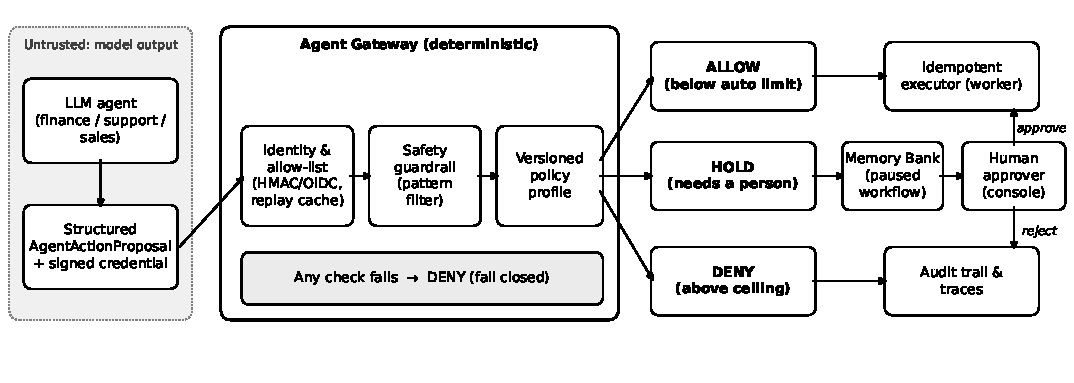
\includegraphics[width=\textwidth]{figures/architecture}
\caption{ApprovalLoop architecture. Model output is untrusted; the gateway checks identity, screens text and evaluates a versioned policy. Only allowed or human-approved proposals reach the idempotent executor; any failed check denies.}
\label{fig:arch}
\end{figure*}

\section{System Design}
\subsection{Proposals and the gateway}
Agents never hold tool credentials. Each emits an \texttt{AgentActionProposal}: agent identity and version, action name, target resource, amount and currency (or parameters such as a discount percentage), recipient, and a free-text justification. The gateway (Fig.~\ref{fig:arch}) processes it in a fixed order:
\begin{enumerate}
\item \emph{Identity.} The agent presents an HMAC-SHA256 token (or a Google OIDC token) whose claims must match the proposal's agent and version. The agent must be registered, active, at the registered version, and allowed to request this action. A per-process cache rejects reused request identifiers.
\item \emph{Screening.} The justification is matched against 23 injection and code-execution patterns and 8 credential formats.
\item \emph{Policy.} The agent's registered profile selects a versioned rule set (Table~\ref{tab:policy}). Unknown profiles, unsupported currencies, non-finite or negative amounts and restricted recipient domains are denied; a missing amount is held for review.
\end{enumerate}
The outcome is \textsc{allow}, \textsc{hold} or \textsc{deny}, with the policy version and the engine's reason recorded verbatim.

\begin{table}[t]
\caption{Policy Profiles in the Reference Implementation}
\label{tab:policy}
\centering
\begin{tabular}{|l|l|l|l|}
\hline
\textbf{Profile} & \textbf{Allow} & \textbf{Hold} & \textbf{Deny} \\
\hline
finance-v3.2.0 (INR) & $<$ 5,000 & 5,000--25,000 & $>$ 25,000 \\
finance-v3.2.0 (USD) & $<$ 50 & 50--250 & $>$ 250 \\
support-v1.1.0 (INR) & $<$ 2,000 & 2,000--10,000 & $>$ 10,000 \\
support-v1.1.0 (USD) & $<$ 20 & 20--100 & $>$ 100 \\
sales-v1.0.0 (discount) & $\le$ 10\% & $>$10--30\% & $>$ 30\% \\
\hline
\end{tabular}
\end{table}

\subsection{Pause, human decision and resumption}
A held proposal is persisted as a paused workflow in a Memory Bank that also stores the action history, every gateway decision and tool results. An operator approves or rejects through an authenticated endpoint; the operator's identity is derived from the credential, never from the request body. Before an approval is claimed, the gateway re-checks that the proposing agent is still active, and approvals older than a configurable time-to-live (24\,h by default) are refused and recorded as expired. The claim is a guarded state transition from \emph{paused} to \emph{approved} or \emph{rejected}, so a second decision on the same action fails.

\subsection{Idempotent execution}
Execution is delegated to a worker with an idempotency key derived from workflow, action and target. The provider records keys it has acknowledged, so a retried or duplicated dispatch returns the original receipt instead of acting twice. A separate scheduled loop that chases stalled expense approvals uses the same discipline: actions are claimed by idempotency key, an LLM may draft only the wording (with a deterministic fallback), and a validator checks recipient, report, amount and state before sending.

\subsection{Operator console}
A React console presents the queue and a single decision sheet per held action. Its central element is a \emph{policy band}: a bar divided into the allow, hold and deny ranges of the evaluating policy version, with a marker at the proposal's amount and an accessible label stating the outcome in words. The agent's justification is shown as an explicitly unverified quotation and rendered as text only. The band is a display copy of backend limits and is hidden for unknown policy versions.

\section{Implementation}
The backend is 4{,}840 lines of Python (FastAPI, Pydantic) in about 30 modules; the console is 1{,}791 lines of TypeScript (React 18). Storage is pluggable: an in-memory repository for development and a Google Cloud Firestore repository for deployment. The project ships a container image for Cloud Run, a scheduler endpoint, 26 test modules, and evaluation scripts. A production start-up check refuses insecure demo authentication and default secrets.

\section{Evaluation}
\subsection{Setup}
All experiments ran in-process against the in-memory repository and a mock execution provider on an Intel x86-64 laptop CPU (family 6, model 154) under Windows 11 with Python 3.10. No network, LLM or Firestore calls were made, so latencies exclude HTTP, database and model inference time. The harness, raw results and figures are in the repository (\texttt{paper/eval}). On the baseline code, the backend test suite passes in full (136 tests) with 80\% line coverage (2{,}489 statements); coverage is lowest for the Firestore repository (31\%) and the HTTP routes (59\%).

\subsection{E1: Policy conformance}
We compared the policy engine against an independent oracle written from the documented thresholds. For each of the five profile--currency combinations we evaluated 8 boundary values (each limit $\pm$0.01, zero and $-$0.01) and 4{,}000 uniform random values over twice the ceiling. All 20{,}040 decisions agreed with the oracle, including all 40 boundary cases. Five fail-closed inputs behaved as specified: unknown profile, unsupported currency and restricted recipient domain were denied, and a missing amount or discount was held. One specification gap surfaced: the documentation describes the sales hold band as ``11--30\%'', leaving discounts between 10\% and 11\% undefined; the code holds them, which we adopted as the reference.

\subsection{E2: Decision latency}
We timed 6{,}000 gateway decisions, 2{,}000 per outcome, in randomly interleaved order after a warm-up. Medians were 0.24, 0.25 and 0.23\,ms for allow (including mock execution), hold (including persistence) and deny; 95th percentiles were 0.38--0.40\,ms and 99th percentiles 0.88--0.95\,ms (Fig.~\ref{fig:latency}). Medians were stable across repeated runs, whereas the 99th percentile varied between runs (0.59--0.95\,ms), consistent with operating-system scheduling noise on a laptop. An earlier, sequential run had suggested that denial was slowest; interleaving showed this to be an ordering artifact. Governance overhead is therefore negligible relative to model inference, which typically takes hundreds of milliseconds or more.

\begin{figure}[t]
\centering
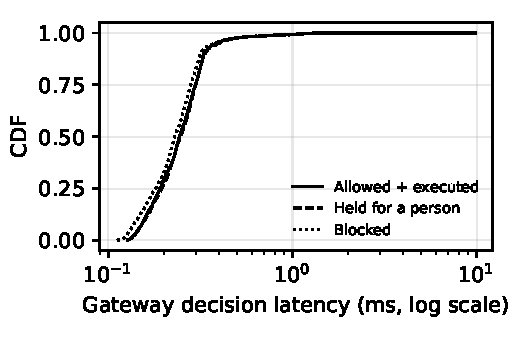
\includegraphics[width=\columnwidth]{figures/latency_cdf}
\caption{Cumulative distribution of in-process gateway decision latency by outcome ($n=2{,}000$ each, interleaved).}
\label{fig:latency}
\end{figure}

\subsection{E3: Approval scalability}
Listing the pending queue and approving an action both locate workflows by scanning every stored workflow. With 100, 1{,}000, 5{,}000 and 10{,}000 stored workflows, the median approval took 0.08, 0.56, 4.0 and 11.9\,ms, and listing the queue 0.06, 0.53, 2.9 and 7.2\,ms (Fig.~\ref{fig:scaling}). Growth is roughly linear. This is acceptable for thousands of workflows in memory, but against a remote store every approval would read the full collection; an index on action identifier and state is required at scale. Section~VIII adds these indexes.

\begin{figure}[t]
\centering
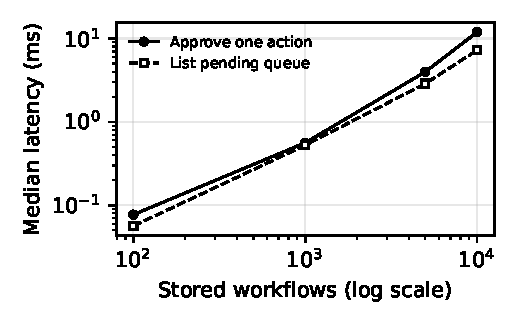
\includegraphics[width=\columnwidth]{figures/approval_scaling}
\caption{Median latency to approve one action and to list the pending queue versus number of stored workflows (30 approvals per point).}
\label{fig:scaling}
\end{figure}

\subsection{E4: Identity attacks}
Table~\ref{tab:identity} lists 12 attack cases against the identity layer, run alongside two controls (a valid request and the first use of a request identifier) that were correctly accepted. Eleven attacks were blocked as intended, including forged signatures, tampered payloads, expired tokens, cross-agent token reuse, stale versions, actions outside the allow-list, replayed request identifiers and disabled agents. The twelfth exposes a design gap: the signed token covers only agent, version and expiry, not the request identifier or the proposal body. An adversary who captures a token can therefore submit arbitrary new proposals with fresh request identifiers until the token expires (5 minutes by default); all five such attempts were accepted. Policy still bounds what those proposals can do, but replay protection as originally implemented does not prevent this; Section~VIII binds tokens to individual requests.

\begin{table}[t]
\caption{Identity Attack Matrix (Gateway, In-Process)}
\label{tab:identity}
\centering
\begin{tabular}{|l|c|}
\hline
\textbf{Case} & \textbf{Blocked} \\
\hline
Missing / malformed token & yes / yes \\
Signed with wrong key & yes \\
Payload tampered (agent\_id) & yes \\
Expired token & yes \\
Token reused by another agent & yes \\
Proposal and credential agent differ & yes \\
Stale agent version & yes \\
Action outside allow-list & yes \\
Replayed request\_id (second use) & yes \\
Disabled agent & yes \\
\textbf{Captured token, fresh request\_ids} & \textbf{no (5/5 accepted)} \\
\hline
\end{tabular}
\end{table}

\subsection{E5: Guardrail detection and containment}
We built a small labeled set: 34 attack texts in five categories and 30 benign justifications, several of which deliberately contain trigger-like words (``system outage'', ``previous instructions on the invoice'', ``bypass road closure''). The set is author-constructed and intended to characterize the filter, not to benchmark it. Detection was complete for verbatim injections (8/8), code and command payloads (6/6) and credential formats (4/4), but near zero for paraphrased injections (0/8) and obfuscations (1/8; only a line-break split was caught, while leetspeak, hyphenation, zero-width characters, a Cyrillic homoglyph, Base64 and Spanish all passed). No benign text was flagged. Overall detection was 19/34 (56\%) (Fig.~\ref{fig:guard}).

To test containment, every attack text was submitted as the justification of a proposal in each of the three finance tiers (102 trials). Detected attacks were denied. The 15 undetected attacks received exactly the outcome their amount dictates: executed automatically below the 5{,}000 limit, held between the limits, denied above the ceiling. No trial reached a more permissive tier than its amount allowed. This is the central empirical result: text screening is weak, but because tiering is a function of structured fields only, a successful injection gains at most the authority the policy already grants for that amount.

\begin{figure}[t]
\centering
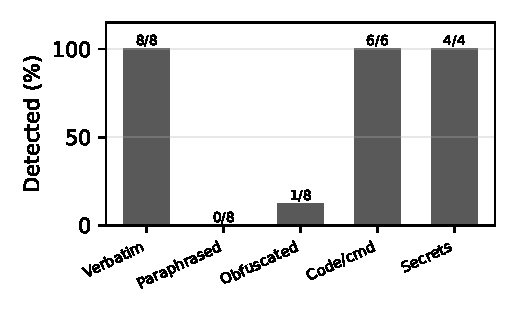
\includegraphics[width=\columnwidth]{figures/guardrail_detection}
\caption{Pattern-based guardrail detection rate by attack category on an author-constructed set (no false positives on 30 benign texts).}
\label{fig:guard}
\end{figure}

\subsection{E6: Concurrent approvals and duplicate execution}
For 2, 4, 8, 16 and 32 threads we ran 40 trials in which all threads, released by a barrier, approved the same held action. In all 200 trials exactly one approval succeeded and exactly one execution occurred. Separately, the project's 1{,}000-report simulation of the expense-reminder loop dispatched 600 actions on the first scheduler tick (350 reminders, 250 escalations, 50 of them to the administrator fallback) and 0 on an immediately overlapping second tick. It recorded 50 race-condition skips, 0 duplicate actions and 0 invalid state transitions in 0.13\,s. This run used the deterministic drafting fallback, as no model key was configured. Both results are single-process: the approval claim is guarded by an in-process lock, and the code itself notes that it is not a Firestore transaction (Section~VIII changes this).

\section{Defects Found During Evaluation}
Reviewing the code and running the experiments surfaced the twelve issues in Table~\ref{tab:defects}. The most serious (D1) was silent: the Firestore repository did not implement workflow listing, the base class supplied a no-op that returned an empty list, and the pending queue, workflow history and the ``agent still active'' check all depend on listing. With the production storage backend, held actions could never be seen or approved, and no test exercised that backend. It was fixed by implementing the method, making all storage operations abstract so that a missing one fails at start-up (D2), and adding tests that run the approval flow through the Firestore repository with an in-memory client; those tests fail when the old behavior is restored. D3 and D4 were fixed by validating amounts explicitly, and D5 by tracking skill files in version control and copying them into the container image. The remaining issues were addressed in a second pass (Section~VIII); Table~\ref{tab:defects} shows the status after both.

\begin{table}[t]
\caption{Defects Identified and Status After Remediation (S = severity: H/M/L; * verified on a simulated store)}
\label{tab:defects}
\centering
\begin{tabular}{|l|p{4.6cm}|c|l|}
\hline
\textbf{ID} & \textbf{Defect} & \textbf{S} & \textbf{Status} \\
\hline
D1 & Firestore workflow listing missing; queue always empty & H & Fixed \\
D2 & Storage base class had silent no-op defaults & M & Fixed \\
D3 & Non-numeric amount caused HTTP 500 & M & Fixed \\
D4 & NaN rejection depended on library version & L & Fixed \\
D5 & Skill files excluded by \texttt{.gitignore} and image & M & Fixed \\
D6 & Approval claim not atomic across instances & H & Fixed* \\
D7 & Token does not bind request\_id or proposal (E4) & M & Fixed \\
D8 & Approve returns success when execution fails & M & Fixed \\
D9 & Linear scans on approve and list (E3) & M & Fixed \\
D10 & Metrics endpoint hard-codes human prompts to 0 & L & Documented \\
D11 & Denied workflows stored with state ``failed'' & L & Fixed \\
D12 & Unpinned test dependencies can crash test runner & L & Fixed \\
\hline
\end{tabular}
\end{table}

D8 matters for the human interface: the approval endpoint returns success with a reason string reporting failed execution, so a client that checks only the status code would tell the operator the payment went through. The console was changed to report such cases as failures, and Section~VIII adds an explicit execution status to the API response.

\section{Remediation and Re-evaluation}
We then addressed the open defects and the aggregate-exposure gap discussed below, and re-ran the same harness on the modified code. Every behavioral change ships with regression tests that fail on the baseline code; the suite grew to 165 tests in 29 modules, with 81\% line coverage of 2{,}658 statements.

\subsection{Changes}
\begin{itemize}
\item \emph{Atomic approval claims (D6).} A decision is prepared on a private copy and committed by compare-and-set, which succeeds only if the stored workflow is still paused: under the repository lock in memory, inside a transaction in Firestore. A test that simulates a second instance with its own lock confirms that the later writer is refused rather than overwriting the first decision.
\item \emph{Request-bound credentials (D7).} A token may carry the request identifier and a SHA-256 digest of the proposal's defining fields, with amounts normalized so that equivalent decimal representations hash identically. The gateway rejects any mismatch and, when configured to (by default in production), any unbound token. The fleet agents always issue bound tokens.
\item \emph{Explicit execution status (D8).} The approval response reports whether execution succeeded, with its receipt or error.
\item \emph{Indexed lookups (D9).} Workflows are indexed by action, state and agent in memory; the Firestore repository uses single-field equality queries.
\item \emph{Daily autonomous-value cap.} Each versioned profile defines a per-agent, per-currency limit on autonomously executed value per UTC day (for \texttt{finance-v3}, 50{,}000 INR or 500 USD). A proposal that would exceed it is held for a person instead of executed. The check and the recording of the decision are serialized, so concurrent proposals cannot overshoot the cap.
\item \emph{De-obfuscating guardrail.} Patterns are additionally matched against Unicode-normalized text with invisible characters removed, common Cyrillic and Greek homoglyphs mapped to Latin, digit substitutions reversed, single-letter spacing collapsed and embedded Base64 decoded.
\item \emph{Smaller fixes.} A distinct \emph{denied} workflow state (D11), bounded test-tool versions (D12), and a corrected description of the reminder-loop metric, which is zero by design (D10).
\end{itemize}

\begin{table}[t]
\caption{Baseline Versus Remediated Implementation (Same Harness)}
\label{tab:remediation}
\centering
\begin{tabular}{|l|l|l|}
\hline
\textbf{Measure} & \textbf{Baseline} & \textbf{After} \\
\hline
Approve, 10{,}000 workflows (median) & 11.9 ms & 0.11 ms \\
List pending, 10{,}000 workflows (median) & 7.2 ms & 0.007 ms \\
Gateway decision (median) & 0.23--0.25 ms & 0.26--0.29 ms \\
Captured-token reuse accepted & 5/5 & 0/5 (bound) \\
Obfuscated injections detected & 1/8 & 7/8 \\
All attacks detected & 19/34 & 25/34 \\
Paraphrased injections detected & 0/8 & 0/8 \\
Benign texts flagged & 0/30 & 0/30 \\
Tier escalations (containment) & 0/102 & 0/102 \\
Double approvals (200 races) & 0 & 0 \\
Policy conformance & 20{,}040/20{,}040 & 20{,}040/20{,}040 \\
Tests; line coverage & 136; 80\% & 165; 81\% \\
\hline
\end{tabular}
\end{table}

\subsection{Results}
Table~\ref{tab:remediation} compares the two versions. Approval latency is now essentially flat, 0.11--0.13\,ms from 100 to 10{,}000 stored workflows (Fig.~\ref{fig:scalecmp}). At 100 workflows it is slightly higher than the baseline's 0.08\,ms, because every claim now copies the workflow before committing. Listing the pending queue fell from 7.2 to 0.007\,ms at 10{,}000 workflows. With binding required, a captured token was rejected on all five reuses.

Detection of obfuscated injections rose from 1 of 8 to 7 of 8; only the Spanish translation passed. Overall detection rose from 19 to 25 of 34, still with no false positives on the 30 benign texts, while paraphrases remained at 0 of 8 (Fig.~\ref{fig:guardcmp}). The containment property was unchanged: none of 102 trials reached a more permissive tier than its amount allowed. The daily cap behaved as specified in the regression tests: of twelve 4{,}999 INR refunds from one agent, the first ten executed and the last two were held; of twenty concurrent 4{,}000 INR proposals, exactly twelve executed (48{,}000 INR). Policy conformance and concurrent-approval results were unchanged. The added work per decision raised median gateway latency from 0.23--0.25 to 0.26--0.29\,ms.

\begin{figure}[t]
\centering
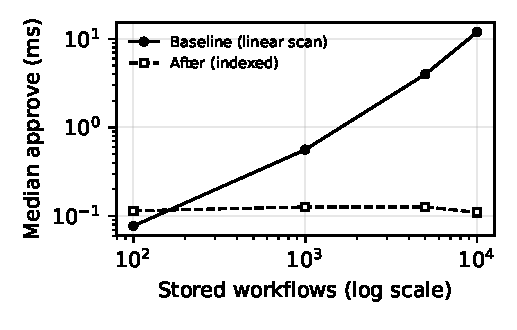
\includegraphics[width=\columnwidth]{figures/approval_scaling_compare}
\caption{Median approval latency versus stored workflows, baseline (linear scan) and after indexing.}
\label{fig:scalecmp}
\end{figure}

\begin{figure}[t]
\centering
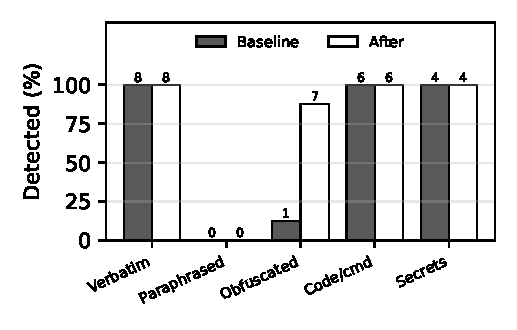
\includegraphics[width=\columnwidth]{figures/guardrail_compare}
\caption{Guardrail detection by category before and after de-obfuscation (numbers above bars are detected cases; benign false positives were 0/30 in both).}
\label{fig:guardcmp}
\end{figure}

\section{Discussion and Limitations}
\textbf{What the evidence supports.} The guarantees G1--G4 held in every experiment on both versions, and the containment result (E5) supports the core design claim: the bound on autonomous loss is set by the policy (per action and, after remediation, per agent per day), independent of how manipulable the model or the text filter is. The same result shows that the guardrail should be viewed as an audit signal and an early exit, not as a security boundary.

\textbf{Per-action and aggregate bounds.} In the baseline, policy limits applied to each proposal independently, so an adversary controlling a model could issue many proposals just under the allow limit. The daily cap now bounds autonomous value per agent and currency per day. It does not limit the number of proposals or the value sent to one recipient, so per-recipient and rate limits remain useful additions.

\textbf{Distributed deployment.} Approval claims now commit by compare-and-set in the store, so two instances cannot both approve the same action. The replay cache and the daily-cap total, however, remain process-local: on a horizontally scaled service each instance keeps its own, so both need a shared store with atomic updates. Request binding is enforced by default only in production, so development deployments still accept unbound tokens.

\textbf{Human factors.} Approval by a person is a control only if the person attends to it \cite{parasuraman2010complacency}. The console shows policy context, unverified justification and checks, but we did not run a user study, and approval fatigue at high hold rates remains unmeasured.

\textbf{Threats to validity.} All measurements are in-process on one machine; network, database and model latency are excluded. The guardrail and identity test sets are small and author-constructed. No real LLM was invoked, so we make no claim about how often a production model would be induced to propose harmful actions. The policy oracle was derived from the same project's documentation, so E1 verifies implementation against intent, not the appropriateness of the limits. The cross-instance claim (D6) was verified against an in-memory stand-in for Firestore that does not model transaction isolation, not against a live multi-instance deployment.

\section{Conclusion and Future Work}
ApprovalLoop demonstrates that a small, deterministic layer between an LLM agent and its tools can enforce per-action monetary limits, durable human approval and at-most-once execution with sub-millisecond overhead, and that these properties do not depend on detecting malicious text. The evaluation also shows that such a system's safety rests on unglamorous details: a missing storage method disabled human approval entirely under the production backend. A second pass fixed most of the defects the evaluation found and was re-measured with the same harness, which we recommend as routine practice for such systems. Future work includes shared, atomic storage for the replay cache and daily caps, a semantic classifier for paraphrased injections, serving policy limits to clients from a single source, evaluation against agent benchmarks such as AgentDojo \cite{debenedetti2024agentdojo} with real models, and a user study of approval decisions.

\begin{thebibliography}{99}
\bibitem{yao2023react} S.~Yao, J.~Zhao, D.~Yu, N.~Du, I.~Shafran, K.~Narasimhan, and Y.~Cao, ``ReAct: Synergizing reasoning and acting in language models,'' in \emph{Proc. Int. Conf. Learning Representations (ICLR)}, 2023.
\bibitem{schick2023toolformer} T.~Schick, J.~Dwivedi-Yu, R.~Dess\`{i}, R.~Raileanu, M.~Lomeli, L.~Zettlemoyer, N.~Cancedda, and T.~Scialom, ``Toolformer: Language models can teach themselves to use tools,'' in \emph{Advances in Neural Information Processing Systems (NeurIPS)}, 2023.
\bibitem{perez2022ignore} F.~Perez and I.~Ribeiro, ``Ignore previous prompt: Attack techniques for language models,'' in \emph{NeurIPS ML Safety Workshop}, 2022, arXiv:2211.09527.
\bibitem{greshake2023indirect} K.~Greshake, S.~Abdelnabi, S.~Mishra, C.~Endres, T.~Holz, and M.~Fritz, ``Not what you've signed up for: Compromising real-world LLM-integrated applications with indirect prompt injection,'' in \emph{Proc. ACM Workshop on Artificial Intelligence and Security (AISec)}, 2023.
\bibitem{liu2024formalizing} Y.~Liu, Y.~Jia, R.~Geng, J.~Jia, and N.~Z. Gong, ``Formalizing and benchmarking prompt injection attacks and defenses,'' in \emph{Proc. USENIX Security Symp.}, 2024.
\bibitem{owasp2023llm} OWASP Foundation, ``OWASP Top 10 for Large Language Model Applications,'' 2023. [Online]. Available: \url{https://owasp.org/www-project-top-10-for-large-language-model-applications/}
\bibitem{nist2023airmf} National Institute of Standards and Technology, ``Artificial Intelligence Risk Management Framework (AI RMF 1.0),'' NIST AI 100-1, Jan. 2023.
\bibitem{debenedetti2025camel} E.~Debenedetti, I.~Shumailov, T.~Fan, J.~Hayes, N.~Carlini, D.~Fabian, C.~Kern, C.~Shi, A.~Terzis, and F.~Tram\`{e}r, ``Defeating prompt injections by design,'' arXiv:2503.18813, 2025.
\bibitem{ruan2024toolemu} Y.~Ruan, H.~Dong, A.~Wang, S.~Pitis, Y.~Zhou, J.~Ba, Y.~Dubois, C.~J. Maddison, and T.~Hashimoto, ``Identifying the risks of LM agents with an LM-emulated sandbox,'' in \emph{Proc. Int. Conf. Learning Representations (ICLR)}, 2024.
\bibitem{debenedetti2024agentdojo} E.~Debenedetti, J.~Zhang, M.~Balunovi\'{c}, L.~Beurer-Kellner, M.~Fischer, and F.~Tram\`{e}r, ``AgentDojo: A dynamic environment to evaluate prompt injection attacks and defenses for LLM agents,'' in \emph{NeurIPS Datasets and Benchmarks Track}, 2024.
\bibitem{saltzer1975protection} J.~H. Saltzer and M.~D. Schroeder, ``The protection of information in computer systems,'' \emph{Proc. IEEE}, vol.~63, no.~9, pp.~1278--1308, 1975.
\bibitem{parasuraman2010complacency} R.~Parasuraman and D.~H. Manzey, ``Complacency and bias in human use of automation: An attentional integration,'' \emph{Human Factors}, vol.~52, no.~3, pp.~381--410, 2010.
\bibitem{helland2012idempotence} P.~Helland, ``Idempotence is not a medical condition,'' \emph{Commun. ACM}, vol.~55, no.~5, pp.~56--65, 2012.
\bibitem{kleppmann2017ddia} M.~Kleppmann, \emph{Designing Data-Intensive Applications}. Sebastopol, CA, USA: O'Reilly Media, 2017.
\end{thebibliography}

\appendix[Reproducing the Results]
From the repository root, with the backend requirements installed:\\
\texttt{PYTHONPATH=backend python paper/eval/run\_evaluation.py}\\
\texttt{python paper/eval/make\_architecture\_figure.py}\\
\texttt{cd backend \&\& PYTHONPATH=. python -m pytest tests}\\
\texttt{PYTHONPATH=backend python evals/run\_large\_scale\_simulation.py}\\
Raw outputs are stored in \texttt{paper/eval/results.json}, \texttt{coverage.txt} and \texttt{large\_scale\_simulation.txt}. These baseline results were produced on the pre-remediation code. The remediated results come from\\
\texttt{PYTHONPATH=backend python paper/eval/run\_evaluation.py -{}-tag after}\\
\texttt{python paper/eval/make\_comparison\_figures.py}\\
and are stored in \texttt{results\_after.json} and \texttt{coverage\_after.txt}.

\end{document}
